\documentclass{article}

\usepackage{listings}
\usepackage{amsmath}
\usepackage{graphicx}
\usepackage{url}
\usepackage{authblk}
\usepackage{array} \setlength{\extrarowheight}{1.5pt}


\begin{document}

\lstset{
%language=C++, % choose the language of the code
basicstyle=\footnotesize, % code font size
numbers=left, % where to put the line-numbers
numberstyle=\footnotesize, % line number font size
stepnumber=1, % the step between two line-numbers.
%backgroundcolor=\color{white}, % choose the background color
frame=single,
framerule=1pt,
captionpos=b, % t or b
showstringspaces=false, % underline spaces within strings
showspaces=false, % show spaces within strings with underscores
showtabs=false, % show tabs within strings with underscores
breaklines=true % Break long lines of code
}

\def\CRC{{\rm CRC}_u}
\def\SCRC{{\rm CRC}_0}
\def\BYTE{{\rm BYTE}}
\def\LCD{{\rm LCD}}
\def\CrcWord{{\rm CrcWord}}

\def\remove#1{}

% -----------------------------------------
\title{Everything we know about CRC but afraid to forget}
\author[1]{Andrew Kadatch}
\affil[1]{Google Inc.}
\author[2]{Bob Jenkins}
\affil[2]{Microsoft Corporation}
\maketitle

\begin{abstract}
  This paper describes a novel interleaved, parallelizeable word-by-word
  CRC computation algorithm which computes $N$-bit CRC ($N \leq 64$) on
  modern Intel and AMD processors in 1.2 CPU cycles per byte, improving
  state of the art over word-by-word 32-bit and 64-bit CRCs (2.1 CPU
  cycles/byte) and classic byte-by-byte CRC computation (6-7 CPU cycles/byte).
  It computes 128-bit CRC in 1.7 CPU cycles/byte.

  CRC implementations are heavily optimized and hard to understand. This
  paper describes CRC algorithms as they evolved over time, splitting
  complex optimizations into a sequence of natural improvements.

  This paper also presents a collection of CRC ``tricks" that we found
  handy on many occassions.
\end{abstract}

\tableofcontents


% -----------------------------------------
\section{Definition of CRC}

Cyclic Redundancy Check (CRC) is a well-known technique that allows the
recipient of a message transmitted over a noisy channel to detect whether
the message has been corrupted.

A message $M = m_0 \dots m_{N-1}$ comprised of $N=|M|$ bits ($m_k \in \{0,
1\}$) may be viewed either as a numeric value
  \begin{align*}
    M = \sum_{k=0}^{N-1} m_k 2^{N-1-k}
  \end{align*}
or as a polynomial of a single variable of degree $(N-1)$
  \begin{align*}
    M(x) = \sum_{k=0}^{N-1} m_k x^{N-1-k}
  \end{align*}
where $m_k \in GF(2) = \{0, 1\}$ and all arithmetic operations on
coefficients are performed modulo 2. For example,
  \begin{align*}
    & \mbox{Addition: }
        (x^3+x^2+x+1) + (x^2+x+1) = x^3+2x^2+2x+2 = x^3, \\
    & \mbox{Subtraction: }
        (x^3+x+1) - (x^2+x) = x^3-x^2+1 = x^3+x^2+1, \\
    & \mbox{Multiplication: }
        (x+1)(x+1) = x^2 + 2x + 1 = x^2 + 1.
  \end{align*}

For a given polynomial $P(x)$ of degree $D=\deg\bigl(P(x)\bigr)$,
$\CRC\bigl(M(x),v(x)\bigr)$ is the reminder from division of $\left(M(x)
\cdot x^D\right)$ by $P(x)$. In practice, a more complex formula is used:
  \begin{align}
    \label{e:crcdefinition}
    \CRC\bigl(M(x), v(x)\bigr)
      = \Bigl(\bigl(v(x)-u(x)\bigr) \cdot x^{|M|} + M(x) \cdot x^D + u(x)\Bigr)
        \bmod P(x),
  \end{align}
where polynomial $P(x)$ of degree $D$ and polynomial $u(x)$ of degree less
than $D$ are fixed.

The use of the non-zero value of $u(x)$ guarantees that the CRC of a sequence
of zeroes is different from zero. That allows detection of insertion of
zeroes in the beginning of a message and replacement of both content of the
message and its CRC value with zeroes. Typically,
  \begin{align}
    \label{e:constdefinition}
    u(x) &= \sum_{k=0}^{D-1} x^k.
  \end{align}

The use of auxilary parameter $v(x)$ allows incremental CRC computation
as shown in section \ref{s:incrementalcrc}.

% -----------------------------------------
\section{Related work}

Cyclic Redundancy Checks (CRCs) were proposed by Peterson and Brown
\cite{Peterson61} in 1961. An efficient table-driven software
implementation which reads and processes data byte by byte was described by
Hill \cite{Hill79} in 1979, Perez \cite{Perez83} in 1983. The ``classic"
byte-by-byte CRC algorithm described in section \ref{s:crcbyte} was
published by Sarwate \cite{DBLP:journals/cacm/Sarwate88} in 1988.

In 1993, Black \cite{Black93} published a method that reads data by words
(described in section \ref{s:crcbyteword}); however, it still computes the
CRC byte by byte in strong sequential order.

In 2001, Braun and Waldvogel \cite{\remove{%braun01fast,
}braun01fast-techreport} briefly outlined a specialized variant of a CRC
that could read input data by words and process them byte by byte -- but,
thanks to the use of multiple tables, different bytes from the input word
could be processed in parallel. In 2002, Ji and Killian \cite{JiKillian02}
provided detailed description and analysis of a nearly identical scheme.
Both solutions were targeted for hardware implementation. In 2005, Kouvanis
and Berry \cite{Kounavis2005\remove{, DBLP:conf/iscc/KounavisB05,
DBLP:journals/tc/KounavisB08}} demonstrated clear performance benefits of
this scheme even when it is implemented in software. A generalized version
of this approach is described in section \ref{s:crcword}.

Surprisingly, until \cite{Gopal2010} we have not seen prior art describing
or utilizing a method of computing a CRC by processing in parallel (in an
interleaved manner to utilize multiple ALUs) multiple input streams
belonging to non-overlapping sections of input data, desribed in section
\ref{s:blockword}.

A novel method of CRC computation that processes in parallel multiple words
belonging to overlapping sections of input data is described in section
\ref{s:multiword}. A special case restricted to the use of 64-bit tables,
64-bit reads, and 32 or 64-bit generating polynomials was implemented by
the authors in February-March 2007 and was used by a couple of Microsoft
products. In 2009, the algorithm was generalized and these limitations were
removed.

The fact that the CRC of a message followed by its CRC is a constant value
which does not depend on the message, described in section
\ref{s:storingcrcafter}, is well known and has been widely used in the
telecommunication industry for long time.

A method of storing a carefully chosen sequence of bits after a message so
that the CRC of a message and the sequence of bits appended to the message
produces predefined result, described in \ref{s:storingcrcafter}, was
implemented in 1990 by Zemtsov \cite{Zemtsov90}.

A method for recomputing a known CRC using a new initial CRC value,
described in section \ref{s:changinginitialvalue}, and the method of
computing a CRC of the concatenation of messages having known CRC values
without touching the actual data, described in section
\ref{s:concatenation}, were implemented by one of the authors in 2005 but
were not published.


% -----------------------------------------
\section{CRC tricks and tips}


% -----------------------------------------
\subsection{Incremental CRC computation} \label{s:incrementalcrc}

The use of an arbitrary initial CRC value $v(x)$ allows computation of a CRC
incrementally. If a message
  $M(x) = M_1(x) \cdot x^{|M_2|} + M_2(x)$
is a concatenation of messages $M_1$ and $M_2$, its CRC may be computed
piece by piece because
  \begin{align}
    \label{e:incremental}
    \CRC\bigl(M(x), v(x)\bigr)
      &= \CRC\Bigl(M_2(x), \CRC\bigl(M_1(x), v(x)\bigr)\Bigr).
  \end{align}

Indeed,
  \begin{align*}
    \CRC(M, v)
      &= \bigl((v-u) x^{|M|} + M x^D + u\bigr) \bmod P = \\
      &= \bigl((v-u) x^{|M_1|+|M_2|} + (M_1 x^{|M_2|} + M_2) x^D + u\bigr) \bmod P = \\
      &= \Bigl(\bigl((v-u) x^{|M_1|} + M_1 x^D \bigr) x^{|M_2|} + M_2 x^D + u\Bigr) \bmod P = \\
      &= \bigl(\CRC(M_1, v) x^{|M_2|} + M_2 x^D + u\bigr) \bmod P = \\
      &= \CRC\bigl(M_2, \CRC(M_1, v)\bigr)
  \end{align*}


% -----------------------------------------
\subsection{Changing initial CRC value} \label{s:changinginitialvalue}

If
  $\CRC\bigl(M(x), v(x)\bigr)$
for some initial value $v(x)$ is known, it is possible to compute
  $\CRC\bigl(M(x), v'(x)\bigr)$
for different initial value $v'(x)$ without touching the value of $M(x)$:
  \begin{align}
    \CRC(M, v')
      &= \CRC(M,v) + \Bigl((v'-v) x^{|M|}\Bigr) \bmod P.
  \label{e:fixv}
  \end{align}

Proof:
  \begin{align*}
    \CRC(M, v')
      &= \bigl((v'-u) x^{|M|} + M x^D + u\bigr) \bmod P = \\
      &= \Bigl(\bigl((v'-u)+(v-v)\bigr) x^{|M|} + M x^D + u\Bigr) \bmod P = \\
      &= \Bigl(\bigl((v-u)+(v'-v)\bigr) x^{|M|} + M x^D + u\Bigr) \bmod P = \\
      &= \Bigl(\bigl((v-u) x^{|M|} + M x^D + u\bigr) + (v'-v) x^{|M|}\Bigr) \bmod P = \\
      &= \CRC(M,v) + \Bigl((v'-v) x^{|M|} \bmod P \Bigr).
  \end{align*}


% -----------------------------------------
\subsection{Concatenation of CRCs} \label{s:concatenation}

If a message
  $M(x) = M_1(x) \cdot x^{|M_2|} + M_2(x)$
is a concatenation of messages $M_1$ and $M_2$, and CRCs of $M_1$, $M_2$
(computed with some initial values $v_1(x)$, $v_2(x)$ respectively) are
known,
 $\CRC\bigl(M(x),v(x)\bigr)$
may be computed without touching contents of the message $M$:
\begin{enumerate}
\item
  Using formula (\ref{e:fixv}), the value of $v'_1 = \CRC(M_1,v)$ may
  be computed from the known $\CRC(M_1,v_1)$ without touching the contents of $M_1$.
\item
  Then, $v'_2 = \CRC(M_2, v'_1)$ may be computed from known $\CRC(M_2,v_2)$
  without touching the contents of $M_2$.
\end{enumerate}
According to (\ref{e:incremental}), $\CRC(M,v) = v'_2$.



% -----------------------------------------
\subsection{In-place modification of CRC-ed message} \label{s:replacement}

Sometimes it is necessary to replace a part of message $M(x)$ in-place and
recompute CRC of modified message $M(x)$ efficiently.

If a message $M=ABC$ is a concatenation of messages $A$, $B$, and $C$, and
$B'(x)$ is new message of the same length as $B(x)$, $\CRC(M')$ of message
$M'=AB'C$ may be computed from known $\CRC(M)$. Indeed,
  \begin{align*}
    M(x)  &= A(x) \cdot x^{|B| + |C|} + B(x) \cdot x^{|C|} + C(x), \\
    M'(x) &= A(x) \cdot x^{|B| + |C|} + B'(x) \cdot x^{|C|} + C(x) = \\
          &= M(x) + \bigl(B'(x) - B(x)\bigr) \cdot x^{|C|},
  \end{align*}
therefore
  \begin{align*}
    &  \CRC\bigl(M'(x),v(x)\bigr) = \\
    &= \CRC\Bigl(M(x) +\bigl(B'(x) - B(x)\bigr) \cdot x^{|C|}\Bigr) = \\
    &= \Bigl(\bigl(v(x)-u(x)\bigr) x^{|M|} + M(x) x^D + \bigl(B'(x) - B(x)\bigr) x^{|C| + D} + u(x)\Bigr) \bmod P(x) \\
    &= \Bigl(\CRC\bigl(M(x),v(x)\bigr) + \bigl(B'(x) - B(x)\bigr) x^{|C| + D}\Bigr) \bmod P(x) = \\
    &= \CRC\bigl(M(x),v(x)\bigr) + \Bigl(\bigl(B'(x) - B(x)\bigr) x^{|C| + D} \bmod P(x)\Bigr).
  \end{align*}

It is easy to see that
  \begin{align*}
    &  \CRC\bigl(B'(x),v(x)\bigr) - \CRC\bigl(B(x),v(x)\bigr) = \\
    &= \bigl(B'(x) - B(x)\bigr) x^{D} \bmod P(x),
  \end{align*}
so
  \begin{align*}
    & \CRC\bigl(M'(x),v(x)\bigr) = \CRC\bigl(M(x),v(x)\bigr) + \Delta \\
  \end{align*}
where
  \begin{align*}
    & \Delta = \Bigl(\CRC\bigl(B'(x),v(x)\bigr) - \CRC\bigl(B(x),v(x)\bigr) \Bigr) x^{|C|} \bmod P(x).
  \end{align*}

% -----------------------------------------
\subsection{Storing CRC value after the message} \label{s:storingcrcafter}

Often $Q(x) = \CRC\bigl(M(x),v(x)\bigr)$ is padded with zero bits until the
nearest byte or word boundary and is transmitted as a sequence of $W$ bits
($W \geq D$) right after the message $M(x)$. This way, the transmitted
message $T(x)$ is the concatenation of $M(x)$ and $Q(x)$ followed by
$(W-D)$ zeroes, and is equal to
  \begin{align*}
    T(x) = M(x) \cdot x^W + Q(x) \cdot x^{W-D}.
  \end{align*}

According to (\ref{e:crcdefinition}), (\ref{e:incremental}) and taking into
account that $Q(x)+Q(x) = 0$ since polynomial coefficient are from $GF(2)$,
$\CRC\bigl(T(x), v(x)\bigr)$ is a constant value which does not depend on
the contents of the message and is equal to
  \begin{align*}
    & \CRC\bigl(T(x), v(x)\bigr) = \\
    & = \CRC\Bigl(Q(x) \cdot x^{W-D}, CRC\bigl(M(x), v(x)\bigr)\Bigr) = \\
    & = \CRC\bigl(Q(x) \cdot x^{W-D}, Q(x)\bigr) = \\
    & = \Bigl(\bigl(Q(x)-u(x)\bigr) \cdot x^W + Q(x)\cdot x^{W-D} \cdot x^D + u(x)\Bigr)
        \bmod P(x) = \\
    & = \Bigl(u(x)\left(1 - x^W\right)\Bigr) \bmod P(x).
  \end{align*}

A more generic solution is to store a $W$-bit long value after the message
such that the CRC of the transmitted message is equal to a predefined value
$R(x)$ (typically $R(x)=0$). The $D$-bit value followed by $(W-D)$ zero
bits that should be stored after $M(x)$ is
  \begin{align*}
    \hat{q}\bigl(Q(x)\bigr) = \Bigl(\bigl(R(x) - u(x)\bigr) x^{-W} - \bigl(Q(x) - u(x)\bigr)\Bigr) \bmod P(x)
  \end{align*}
where $x^{-W}$ is the multiplicative inverse of $x^W \bmod P(x)$ which
exists if $P(x)$ is not divisble by $x$ and may be found by the extended
Euclidean algorithm \cite{Hasan01}:
  \begin{align*}
    & \CRC\Bigl(\hat{q}\bigl(Q(x)\bigr)x^{W-D}, CRC\bigl(M(x), v(x)\bigr)\Bigr) = \\
    & = \CRC\Bigl(\hat{q}\bigl(Q(x)\bigr)x^{W-D}, Q(x)\Bigr) = \\
    & = \Bigl(\bigl(Q(x)-u(x)\bigr) \cdot x^W + \hat{q}\bigl(Q(x)\bigr) \cdot x^{W-D} \cdot x^D + u(x)\Bigr)
          \bmod P(x) = \\
    & = R(x).
  \end{align*}


% -----------------------------------------
\section{Efficient software implementation}

% -----------------------------------------
\subsection{Mapping bitstreams to hardware registers}

For little-endian machines (assumed from now on), the result of loading of
a $D$-bit word from memory into hardware register matches the expectations:
the 0-th bit of the 0-th byte becomes the 0-th (least significant) bit of
the word corresponding to $x^{(D-1)}$.

For example, the 32-bit sequence of 4 bytes 0x01, 0x02, 0x03, 0x04
(0x04030201 when loaded into a 32-bit hardware register) corresponds to the
polynomial
  \begin{align*}
    \left(x^{31} + x^{22} + x^{15} + x^{14} + x^{5}\right).
  \end{align*}

Addition and subtraction of polymonials with coefficients from $GF(2)$ is
the bitwise XOR of their coefficients. Multiplication of a polynomial by
$x$ is achieved by logical right shift of register contents by 1 bit. If a
shift operation causes a carryover, the resulting polynomial has degree
$D$.

Polynomials of degree less than $D$ whose coefficients are recorded using
exactly $D$ bits irrespective of actual degree of the polynomial will be
called {\it $D$-normalized}.

Whenever possible -- and unless mentioned explicitly -- all polynomials
will be represented in $D$-normalized form.

Since the generating polynomial $P(x)$ is of degree $D$ and has $(D+1)$
coefficients, it does not fit into the $D$-bit register. However, its most
significant coefficient is guaranteed to be 1 and may be implied
implicitly.

% -----------------------------------------
\subsection{Multiplication of $D$-normalized polynomials} \label{s:shiftandadd}

Multiplication of two $D$-normalized polynomials may be accomplished by
traditional bit-by-bit, shift-and-add multiplication. This is adequate if
performance is not a concern. Sample code is given in listing
\ref{l:MulNormalizedPoly}.

\begin{figure}
\begin{lstlisting}[caption={Multiplication of normalized polynomials},label={l:MulNormalizedPoly}]
// "a" and "b" occupy D least significant bits.
Crc Multiply(Crc a, Crc b) {
  Crc product = 0;
  Crc bPowX[D];  // bPowX[k] = (b * x**k) mod P
  bPowX[0] = b;
  for (int k = 0; k < D; ++k) {
    // If "a" has non-zero coefficient at x**k,
    // add ((b * x**k) mod P) to the result.
    if (((a & (1 << (D-k)) != 0) product ^= bPowX[k];

    // Compute bPowX[k+1] = (b ** x**(k+1)) mod P.
    if (bPowX[k] & 1) {
      // If degree of (bPowX[k] * x) is D, then
      // degree of (bPowX[k] * x - P) is less than D.
      bPowX[k+1] = (bPowX[k] >> 1) ^ P;
    } else {
      bPowX[k+1] = bPowX[k] >> 1;
    }
  }
  return product;
}
\end{lstlisting}
\end{figure}

% -----------------------------------------
\subsection{Multiplication of unnormalized polynomial}

During initialization of CRC tables it may be necessary to multiply
$d$-normalized polynomial $v(x)$ of a degree $d \neq D$ by a $D$-normalized
polynomial. It may be accomplished by representing the operand as a sum of
weighted polynomials of degree of no more than $(D-1)$, then calling
$Multiply()$ function repeatedly as shown in listing
\ref{l:MulUnnormalizedPoly}.

\begin{figure}
\begin{lstlisting}[caption={Multiplication of unnormalized polynomial},label={l:MulUnnormalizedPoly}]
// "v" occupies "d" least signficant bits.
// "m" occupies D least significant bits.
Crc MultiplyUnnormalized(Crc v, int d, Crc m) {
  Crc result = 0;
  while (d > D) {
    Crc temp = v & ((1 << D) - 1);
    v >>= D;
    d -= D;
    // XpowN returns (x**N mod P(x)).
    result ^= Multiply(temp, Multiply(m, XpowN(d)));
  }
  result ^= Multiply(v << (D - d), m);
  return result;
}
\end{lstlisting}
\end{figure}


% -----------------------------------------
\subsection{Computing powers of $x$} \label{s:mulpown}

Often (see sections \ref{s:changinginitialvalue}, \ref{s:concatenation},
\ref{s:storingcrcafter}) it is necessary to compute $x^N \bmod P(x)$ for
very large values of $N$. This may be accomplished in
$O\bigl(\log(N)\bigr)$ time.

Consider the binary representation of $N$:
  \begin{align*}
    N = \sum_{k=0}^K n_k 2^k
  \end{align*}
where $n_k \in \{0, 1\}$. Then
  \begin{align}
    x^N &= x^{\sum n_k 2^k}
         = \prod_{k=0}^K x^{n_k 2^k}
         = \prod_{n_k != 0} x^{2^k} \label{e:pow2k}
  \end{align}
and may be computed using no more than
    $\left(\left\lfloor \log_2(N) \right\rfloor + 1\right)$
multiplications of polynomials of degree less than $D$ provided known
values of
  \begin{align}
    Pow2k(k) = x^{2^k} \bmod P(x).
  \end{align}

Values of $Pow2k(k)$ may be computed iteratively using one multiplication
$\bmod P(x)$ per iteration:
  \begin{align*}
    Pow2k(0) &= 0, \\
    Pow2k(k + 1)
      &= x^{2^{k+1}} \bmod P(x) = \\
      &= x^{2 \cdot 2^k} \bmod P(x) = \\
      &= \left(x^{2^k}\right)^2 \bmod P(x) = \\
      &= \Bigl(Pow2k(k-1)\Bigr)^2 \bmod P(x).
  \end{align*}

% -----------------------------------------
\subsection{Simplified CRC}

It is sufficient to be able to compute
  \begin{align}
    \SCRC\bigl(M(x), v(x)\bigr)
      &= \Bigl(v(x) \cdot x^{|M|} + M(x) \cdot x^D\Bigr)
        \bmod P(x), \label{e:simplifiedcrc}
  \end{align}
since
  \begin{align*}
    \CRC\bigl(M(x),v(x)\bigr) &= \SCRC\bigl(M(x), v(x) - u(x)\bigr) + u(x),
  \end{align*}
$\CRC\bigl(M(x),v(x)\bigr)$ of message $M = M_1 \ldots M_K$ may be computed
incrementally using $\SCRC$ instead of $\CRC$:
  \begin{align*}
    v_0(x) &= v(x) - u(x), \\
    v_k(x) &= \SCRC\bigl(M_k(x),v_{k-1}(x)\bigr), \\
    \CRC(M(x), v(x)) &= v_K + u(x).
  \end{align*}


% -----------------------------------------
\subsection{Computing a CRC byte by byte} \label{s:crcbyte}

If $M(x)$ is $W$-bit value (typically, $W=8$) and
$\deg\bigl(v(x)\bigr) < D$, by definition (\ref{e:simplifiedcrc})
  \begin{align*}
    \SCRC\bigl(M(x), v(x)\bigr)
      = \Bigl(v(x) \cdot x^W + M(x) \cdot x^D\Bigr) \bmod P(x).
  \end{align*}

When $D \leq W$,
\begin{align}
  \SCRC\bigl(M(x), v(x)\bigr)
    &= \Bigl(v(x) \cdot x^W + M(x) \cdot x^D\Bigr) \bmod P(x) = \nonumber \\
    &= \Bigl(\bigl(v(x) \cdot x^{W-D} + M(x)\bigr) \cdot x^D\Bigr) \bmod P(x), \label{e:crcbytetable2}
\end{align}
which may be obtained via single lookup into precomputed table $T$ of size
$2^W$ such that $T[i] = \bigl(i(x) \cdot x^D)\bigr) \bmod P(x)$ since
$\deg\bigl(v(x) \cdot x^{W-D} + M(x)\bigr) < W$.

$D$-normalized representation of $v(x)$ occupies $D$ least significant bits
and is equal to $\left(v(x) \cdot x^{W-D}\right)$ when viewed as
$W$-normalized representation which is required to form $W$-bit index into
a table of $2^W$ entries. Therefore, explicit multiplication of $v(x)$ by
$x^{W-D}$ in formula (\ref{e:crcbytetable2}) is not required.

When $D \geq W$, $v(x)$ may be represented as
  \begin{align*}
    v(x) = v_L(x) + v_H(x) \cdot x^{D-W}
  \end{align*}
where
  \begin{align*}
    v_H(x) &= \left\lfloor\frac{v(x)}{x^{D-W}}\right\rfloor,
        &\deg\bigl(v_H(x)\bigr) &< W, \\
    v_L(x) &= v(x) \bmod x^{D-W},
        &\deg\bigl(v_L(x)\bigr) &< D-W.
  \end{align*}

Since $\deg\bigl(v_L(x) \cdot x^W \bigr) < D$, $\Bigl(v_L(x) \cdot
x^W\Bigr) \bmod P(x) = v_L(x) \cdot x^W$. Therefore,
  \begin{align}
    & \SCRC\bigl(M(x), v(x)\bigr) = \nonumber \\
      &= \Bigl(v(x) \cdot x^W + M(x) \cdot x^D\Bigr) \bmod P(x) = \nonumber \\
      &= \Bigl(\bigl(v_L(x) + v_H(x) \cdot x^{D-W}\bigr)\cdot x^W + M(x) \cdot x^D\Bigr) \bmod P(x) = \nonumber \\
      &= \Bigl(v_L(x) \cdot x^W + \bigl(v_H(x) + M(x)\bigr) \cdot x^D\Bigr) \bmod P(x) = \nonumber \\
      &= \Bigl(v_L(x) \cdot x^W + \bigl(v_H(x) + M(x)\bigr) \cdot x^D\Bigr) \bmod P(x) = \nonumber \\
      &= \Bigl(v_L(x) \cdot x^W\Bigr) \bmod P(x) + \Bigl(\bigl(v_H(x) + M(x)\bigr) \cdot x^D \Bigr) \bmod P(x) = \nonumber \\
      &= \Bigl(v_L(x) \cdot x^W\Bigr) + \mbox{MulByXpowD}\bigl(v_H(x) + M(x)\bigr), \label{e:crcbyte}
  \end{align}
where
  \begin{align}
    \mbox{MulByXpowD}\bigl(a(x)\bigr) = \bigl(a(x) \cdot x^D \bigr) \bmod P(x). \label{e:crcbytetable}
  \end{align}

The value of $\bigl(v_L(x) \cdot x^W\bigr)$ may be computed by shifting
$v(x)$ by $W$ bits and discarding $W$ carry-over zero bits.

Since $\deg\bigl(v_H(x) + M(x)\bigr) < W$, the value of
$\mbox{MulByXpowD}\bigl(v_H(x) + M(x)\bigr)$ may be obtained using
precomputed table containing $2^W$ entries.

The classic table-driven, byte-by-byte CRC computation \cite{Perez83,
DBLP:journals/cacm/Sarwate88} implementing formulas
(\ref{e:crcdefinition}), (\ref{e:incremental}), (\ref{e:crcbytetable2}),
(\ref{e:crcbyte}), and (\ref{e:crcbytetable}) for $W=8$ is given in listing
\ref{l:CrcByte}.

\begin{figure}
\begin{lstlisting}[caption={Computing CRC byte by byte},label={l:CrcByte}]
Crc CrcByte(Byte value) {
  return MulByXpowD[value];
}
Crc CrcByteByByte(Byte *data, int n, Crc v, Crc u) {
  Crc crc = v ^ u;
  for (int i = 0; i < n; ++i) {
    Crc ByteCrc = CrcByte(crc ^ data[i]);
    crc >>= 8;
    crc ^= ByteCrc;
  }
  return (crc ^ u);
}
void InitByteTable() {
  for (int i = 0; i < 256; ++i) {
    MulByXPowD[i] = MultiplyUnnormalized(i, 8, XpowN(D));
  }
}
\end{lstlisting}
\end{figure}

Experience shows that computing CRC byte by byte is rather slow and,
depending on a compiler and input data size, takes $6-8$ CPU cycles per
byte on modern 64-bit CPU for $D <= 64$. There are two reasons for it:

\begin{enumerate}
\item
  Reading data 8 bits at a time is not the most efficient data access
  method on 64-bit CPU.
\item
  Modern CPUs have multiple ALUs and may execute 3-4 instructions per CPU
  cycles provided the instructions handle independent data flows. However,
  byte-by-byte CRC contains only one data flow. Futhermore, most
  instructions use the result from the previous instruction, leading to CPU
  stalls because of result propagation delays.
\end{enumerate}


% -----------------------------------------
\subsection{Rolling CRC} \label{s:rollingcrc}

Given a set of messages $M_k=m_{k} \ldots m_{k+N-1}$ where $m_k$ are
$W$-bit symbols and $N$ is fixed (i.e. each next message is obtained by
removing first symbol and appending new one), $C_{k+1} = \CRC(M_{k+1}, v)$
may be obtained from known $C_k = \CRC(M_k, v)$ and symbols $m_k$ and
$m_{k+N}$ only, without the need to compute CRC of entire message
$M_{k+1}$. This property may be utilized to efficiently compute a set of
rolling Rabin fingerpints.

Since $M_{k+1}(x) = M_k(x) x^W - m_{k}(x) x^{NW} + m_{k+N}(x)$,
  \begin{align*}
    & C_{k+1}(x) = \CRC\bigl(M_{k+1}(x), v(x)\bigr) = \\
    &= \left(\bigl(v(x)-u(x)\bigr) x^{NW} + u(x) + \sum_{n=0}^{N-1} m_{k+1+n}(x) x^{D+W(N-1-n)} \right) \bmod P(x) = \\
    &= F\bigl(C_k(x), m_{k+N}(x)\bigr) + G\bigl(m_k(x)\bigr),
  \end{align*}
where
  \begin{align*}
    & F\bigl(C_k(x), m_{k+N}(x)\bigr) = \Bigl(C_k(x) x^W + m_{k+N}(x) x^D\Bigr) \bmod P, \\
    & G\bigl(m_k(x)\bigr) = \Bigl(\bigl(\bigl(v(x)-u(x)\bigr) x^{NW} + u\bigr) (1 - x^W) - m_k(x) x^{D+NW} \Bigr) \bmod P
  \end{align*}
are polynomials of degree less than $D$.

$G\bigl(m_{k-1}(x)\bigr)$ may be computed easily via a single lookup
in a table of $2^W$ entries indexed by $m_k$.

Computation of $F\bigl(C_k(x), m_{k+N}(x)\bigr)$ may be implemented as
described in section \ref{s:crcbyte} and requires one bitwise shift, one
bitwise XOR, and one lookup into a precomputed table containing $2^W$
entries.


% -----------------------------------------
\subsection{Reading multiple bytes at a time} \label{s:crcbyteword}

One straightforward way to speed up byte-by-byte CRC computation is to read
$W > 8$ bits at once. Unfortunately, this is the path of very rapidly
diminishing return as the size of the MulByPowD table increases with $W$
exponentially. From practical perspective, it is extremely desirable to
ensure that the MulByPowD table fits into the L1 cache (32-64KB), otherwise
table entry access latency sharply increases from 3-4 CPU cycles (L1 cache)
to 15-20 CPU (L2 cache).

The value of $\mbox{MulByXpowD}\bigl(v(x)\bigr)$ may be computed
iteratively using a smaller table because
  \begin{align}
    \mbox{MulByXpowD}\bigl(v(x)\bigr)
      = v(x) \cdot x^D \bmod P(x)
      = \SCRC\bigl(v(x), 0\bigr) \label{e:readwordatonce}
  \end{align}
and therefore may be computed using formulas (\ref{e:incremental}) and
(\ref{e:crcbyte}) for smaller values of $W'$.

\cite{Black93} provided the implementation for $W=32$ and $W'=8$. Our more
general implementation was faster than byte-by-byte CRC but not
substentially: the improvement was in 20-25\% range. However, the result is
still important -- it demonstrates that reading input data per se is not a
bottleneck.


% -----------------------------------------
\subsection{Computing a CRC word by word} \label{s:crcword}

The value of $\mbox{MulByXpowD}\bigl(v(x)\bigr)$ may be computed using
multiple smaller tables instead of one table. Given that
$\deg\bigl(v(x)\bigr) < W$, $v(x)$ may be represented as a weighted
sum of polynomials $v_k(x)$ such that $\deg\bigl(v_k(x)\bigr) < B$:
  \begin{align*}
    v(x) = \sum_{k=0}^{K-1} v_k(x) \cdot x^{(K-1-k)B},
  \end{align*}
where $K = \lceil W/B \rceil$ and
  \begin{align*}
    v_k(x) = \left\lfloor \frac{v(x)}{x^{(K-1-k)B}} \right\rfloor \bmod x^B.
  \end{align*}

Consequently,
  \begin{align}
    \mbox{MulByXpowD}\bigl(v(x)\bigr)
      &= v(x) \cdot x^D \bmod P(x) = \nonumber \\
      &= \left(\sum_{k=0}^{K-1} v_k(x) \cdot x^{(K-1-k)B}\right) \cdot x^D \bmod P(x) = \nonumber \\
      &= \sum_{k=0}^{K-1} \left(v_k(x) \cdot x^{(K-1-k)B+D} \bmod P(x)\right) = \nonumber \\
      &= \sum_{k=0}^{K-1} \mbox{MulWordByXpowD}\bigl(k, v_k(x)\bigr), \label{e:crcword}
  \end{align}
where the values of
  \begin{align}
    \mbox{MulWordByXpowD}\bigl(k, v_k(x))\bigr) = v_k(x) \cdot x^{(K-1-k)B+D} \bmod P(x) \label{e:crcwordtable}
  \end{align}
may be obtained using $K$ precomputed tables. Given that
$\deg\bigl(v_k(x)\bigr) < B$, each table should contain $2^B$
entries.

A sample implementation of formulas (\ref{e:crcdefinition}),
(\ref{e:incremental}), (\ref{e:crcword}), and (\ref{e:crcwordtable}) is
given in listing \ref{l:CrcWord} using $B=8$ and assuming that $W$ is a
multiple of 8.

\begin{figure}
\begin{lstlisting}[caption={Computing CRC word by word},label={l:CrcWord}]
Crc CrcWord(Word value) {
  Crc result = 0;
  // Unroll this loop or let compiler do it.
  for (int byte = 0; byte < sizeof(Word) / 8; ++byte) {
    result ^= MulWordByXpowD[byte][(Byte) value];
    value >>= 8;
  }
  return result;
}
Crc CrcWordByWord(Word *data, int n, Crc v, Crc u)
  Crc crc = v ^ u;
  for (int i = 0; i < n; ++i) {
    Crc WordCrc = CrcWord(crc ^ data[i]);
    if (sizeof(Crc) <= sizeof(Word)) {
      crc = WordCrc;
    } else {
      crc >>= 8;
      crc ^= WordCrc;
    }
  }
  return (crc ^ u);
}
void InitWordTables() {
  for (int byte = 0; byte < sizeof(Word) / 8; ++byte) {
    // (K-1-k)*B + D = (W/8-1-byte)*8 + D = D - 8 + W - 8*byte.
    Crc m = XpowN(D - 8 + sizeof(Word)*8 - 8*byte);
    for (int i = 0; i < 256; ++i) {
      MulWordByXpowD[byte][i] =MultiplyUnnormalized(i, 8, m);
    }
  }
}
\end{lstlisting}
\end{figure}

CrcWordByWord\footnote{The variant presented in this paper is more general
than ``slicing" described in \cite{Kounavis2005\remove{,
DBLP:conf/iscc/KounavisB05, DBLP:journals/tc/KounavisB08}}. Sample
implementation given in listing \ref{l:CrcWord} does not include one subtle
optimization implemented in \cite{Kounavis2005\remove{,
DBLP:conf/iscc/KounavisB05, DBLP:journals/tc/KounavisB08}} as it was found
to be counter-productive.} with $W=64$ uses only 2.1-2.2 CPU cycles/byte on
modern 64-bit CPUs (our implementation is somewhat faster than the one
described in \cite{Kounavis2005\remove{, DBLP:conf/iscc/KounavisB05,
DBLP:journals/tc/KounavisB08}}). It solves the problem with data access
and, to lesser degree, allows instruction level parallelism: in the middle
of the unrolled main loop of CrcOfWord function the CPU may process
multiple bytes in parallel.

However, this solution is still imperfect -- the beginning of computation
contends for a single source of data (variable $value$), and the end of
computation contends for a single destination (variable $result$). Further
improvement requires processing of multiple independent data streams in
interleaved manner so that when computation of one data flow path is
stalled the CPU may proceed with another one.

% -----------------------------------------
\subsection{Processing non-overlapping blocks in parallel} \label{s:blockword}

Straighforward pipepiling may be achieved by spliting the input message
$M(x)=M_0(x) \ldots M_{N-1}(x)$ into $N$ blocks $M_k(x)$ of approximately
the same size and computing CRC of each block in an interleaved manner,
concatenating CRCs of individual blocks in the end. A sample implementation
is given in listing \ref{l:CrcWordBlock}.

\begin{figure}
\begin{lstlisting}[caption={Processing non-overlapping blocks in parallel},label={l:CrcWordBlock}]
// Processes N stripes of StripeWidth words each
// word by word, in an interleaved manner.
Crc CrcWordByWordBlocks(Word *data, Crc v, Crc u) {
  assert(n % (N * StripeWidth) == 0);
  // Use N local variables instead of the array.
  Crc crc[N];
  // Initialize the CRC value for each stripe.
  crc[0] = v ^ u;
  for (int stripe = 1; stripe < N; ++stripe)
    crc[i] = 0 ^ u;
  // Compute each stripe's CRC.
  for (int i = 0; i < StripeWidth; ++i) {
    // Compute multiple CRCs in interleaved manner.
    Word buf[N];
    for (int stripe = 0; stripe < N; ++stripe) {
      buf[i] =
        crc[stripe] ^ data[i + stripe * StripeWidth];
      if (D > sizeof(Word) * 8) {
        crc[stripe] >>= D - sizeof(Word) * 8;
      } else {
        crc[stripe] = 0;
      }
    }
    for (int byte = 0; byte < sizeof(Word) / 8; ++byte) {
      for (int stripe = 0; stripe < N; ++stripe) {
        crc[stripe] ^=
          MulWordByXpowD[byte][(Byte) buf[stripe]];
        buf[stripe] >>= 8;
      }
    }
  }
  // Combine stripe CRCs.
  for (int stripe = 1; stripe < N; ++stripe) {
    crc[0] = ChangeStartingValue(
                crc[stripe], StripeWidth, 0, crc[0]);
  }
  return (crc[0] ^ u);
}
\end{lstlisting}
\end{figure}

A tuned implementation of $CrcWordByWordBlocks$ is capable of processing
data at 1.3-1.4 CPU cycles/byte on sufficiently large (64KB and more)
inputs, which is noticeably better that 2.1-2.2 CPU cycles/byte delivered
by word by word CRC computation. It is a good sign that it is a move in
right direction.

The drawbacks of this approach are obvious: it does not work well with
small inputs -- the cost of CRC concatentation becomes a bottleneck, -- and
it may be susceptible to false cache collisions caused by cache line
aliasing.

If the cost of CRC concatenation was not a problem, cache pressure could be
mitigated with the use of very narrow stripes. The code in question, lines
33-37 of listing \ref{l:CrcWordBlock} which combine CRCs of individual
stripes, iteratively computes
  \begin{align*}
    \mbox{crc}_0(x) = \mbox{crc}_k(x) + \Bigl(\mbox{crc}_0 \cdot x^{8S} \bmod P(x)\Bigr)
  \end{align*}
for $k = 1, \ldots, N-1$ where $N$ and $S$ are the number and the width of
the stripes respectively. It may be rearranged as
  \begin{align*}
    \mbox{crc}_0(x) = \sum_{k = 0}^{N-1} \Bigl(\mbox{crc}_{K-1-k} \cdot x^{8kS} \bmod P(x)\Bigr).
  \end{align*}

Explicit multiplication by $x^{8kS}$ may be avoided by moving it into preset
tables
  \begin{align*}
    \mbox{MulWordByXPowD}_k(n) = \mbox{MulWordByXPowD}(n) \cdot x^{kS} \bmod P(x).
  \end{align*}
that are used to compute $crc'_k(x) = \mbox{crc}_k(x) \cdot x^{8kS}$, so that
  \begin{align*}
    \mbox{crc}_0(x) = \sum_{k = 0}^{N-1} crc'_k.
  \end{align*}

Unfortunately, this approach alone does not help because
\begin{enumerate}
\item
  It increases the memory footprint of MulWordByXPowD by factor of $N$.
  Once the cumulative size of $\mbox{MulWordByXPowD}_k$ tables exceeds the
  size of L1 cache (32-64KB), the cost of memory access to multiplication
  table data increases from 3-4 CPU cycles to 15-20, eliminating all
  performance gains achieved by reducing the number of table operations.
\item
  It is still necessary to combine all $N$ values of $\mbox{crc}_k$ into
  $\mbox{crc}_0$ at the end of the CRC computation.
\end{enumerate}


% -----------------------------------------
\subsection{Interleaved word-by-word CRC} \label{s:multiword}

% -----------------------------------------
\subsubsection{Parallelizing CRC computation} \label{s:parallelizing}

Assume that input message $M$ is the concatenation of $K$ groups $g_k$, and
each group $g_k$ is concatenation of $N$ $W$-bit long words:
  \begin{align*}
    M(x) &= \sum_{k=0}^{K-1} g_k(x) \cdot x^{(K-1-k)NW}, \\
    g_k(x) &= \sum_{n=0}^{N-1} m_{k, n} \cdot x^{(N-1-n)W}.
  \end{align*}

Input message $M(x)$ may be represented as
  \begin{align}
    M(x)
      &= \sum_{k=0}^{K-1} g_k(x) \cdot x^{(K-1-k)NW} = \nonumber \\
      &= \sum_{k=0}^{K-1} \left(\sum_{n=0}^{N-1} m_{k, n} \cdot x^{(N-1-n)W} \right) \cdot x^{(K-1-k)NW} = \nonumber \\
      &= \sum_{n=0}^{N-1} \left(\sum_{k=0}^{K-1} m_{k, n} \cdot x^{(K-1-k)NW}\right) \cdot x^{(N-1-n)W} = \nonumber \\
      &= \sum_{n=0}^{N-1} M_n(x) \cdot x^{(N-1-n)W} \label{e:splitbyword}
  \end{align}
where
  \begin{align*}
    M_n(x)
      &= \sum_{k=0}^{K-1} m_{k, n} \cdot x^{(K-1-k)NW}.
  \end{align*}

In other words, $M_n$ is concatenation of $n$-th $W$-bit word from $g_0$
followed by $(N-1)W$ zero bits, then $n$-th word from $g_1$ followed by
$(N-1)W$ zero bits, etc., ending up with $n$-th word from last group
$g_{K-1}$.

Appending $(N-1)W$ zero bits to $M_n$ yields $M'_n(x) = M_n(x) \cdot
x^{(N-1)W} $ which may be viewed as the concatenation of $K$ $NW$-bit
groups $f_{k}$:
  \begin{align*}
    M'_n(x)
      &= M_n(x) \cdot x^{(N-1)W}
      = \sum_{k=0}^{K-1} f_{k, n} \cdot x^{(K-1-k)NW}, \\
    f_{k, n}(x) &= m_{k, n}(x) \cdot x^{(N-1)W}, \\
  \end{align*}
so
  \begin{align}
    M(x)
      &= \sum_{n=0}^{N-1} M_n(x) \cdot x^{(N-1-n)W} \nonumber \\
      &= \sum_{n=0}^{N-1} M'_n(x) \cdot x^{-(N-1)W} \cdot x^{(N-1-n)W} \nonumber \\
      &= \sum_{n=0}^{N-1} M'_n(x) \cdot x^{-nW}. \label{e:mdash}
  \end{align}

According to (\ref{e:incremental}),
  $v_{K, n}(x) = \SCRC\bigl(M'_n(x), v_{0, n}(x)\bigr)$
may be computed incrementally:
  \begin{align}
    v_{k+1, n}(x)
      &= \SCRC\bigl(f_{k, n}(x), v_{k, n}(x)\bigr) = \nonumber \\
      &= \SCRC\bigl(m_{k, n}(x) \cdot x^{(N-1)W}, v_{k, n}(x)\bigr) = \nonumber \\
      &= \Bigl(v_{k, n}(x) \cdot x^{NW} + m_{k, n}(x) \cdot x^{(N-1)W} \cdot x^D \Bigr) \bmod P(x) = \nonumber \\
      &= \Bigl(v_{k, n}(x) \cdot x^W + m_{k, n}(x) \cdot x^D \Bigr) \cdot x^{(N-1)W} \bmod P(x) = \label{e:crcwordnmultiply} \\
      &= \mbox{CrcWordN}\bigl(m_{k, n}(x), v_{k, n}(x)\bigr). \label{e:crcwordn}
  \end{align}

This approach:
\begin{enumerate}
\item
  Creates $N$ independent data flows: computation of $v_{k, 0}, \ldots,
  v_{k, N-1}$ may be performed truly in parallel. There are no contentions
  on a single data source or destination like those the word-by-word CRC
  computation described in section \ref{s:crcword} suffered from.
\item
  Input data is accessed sequentially. Therefore, the load on cache
  subsystem and false cache collisions are  minimal. Thus, the performance
  bottlenecks of approach described in \ref{s:blockword} are eliminated.
\end{enumerate}


% -----------------------------------------
\subsubsection{Combining individual CRCs} \label{s:combine}

Once $v_{K, n}(x) = \SCRC\bigl(M'_n(x), v_{0, n}(x)\bigr)$ are computed starting with
  \begin{align*}
    v_{0, 0} &= v(x), \\
    v_{0, n} &= 0, n \geq 1,
  \end{align*}
by definition (\ref{e:simplifiedcrc}) of $\SCRC$ and relationship (\ref{e:mdash}),
  \begin{align}
    \SCRC\bigl(M(x), v(x)\bigr)
      &= \SCRC\left(\sum_{n=0}^{N-1} M'_n(x) \cdot x^{-nW}, v(x)\right) = \nonumber \\
      &= \sum_{n=0}^{N-1} \SCRC\bigl(M'_n(x) \cdot x^{-nW}, v_{0, n}(x) \bigr) = \nonumber \\
      &= \sum_{n=0}^{N-1} \SCRC\bigl(M'_n(x), v_{0, n}(x) \bigr) \cdot x^{-nW} = \nonumber \\
      &= \sum_{n=0}^{N-1} v_{K, n}(x) \cdot x^{-nW}. \label{e:multiwordcrc1}
  \end{align}

Even though this step is performed only once per input message, it still
requires $(N-1)$ non-trivial multiplications modulo $P(x)$ negatively
affecting the performance on small input messages. Also,
(\ref{e:multiwordcrc1}) uses the multiplicative inverse of $x^{nW}$ modulo
$P(x)$ which does not exists when $P(x) \bmod x = 0$.

There is more efficient and elegant solution. Assume that $M(x)$ is
followed by one more group $g_K(x)$. Then
  \begin{align}
    & \SCRC\bigl(M(x) \cdot x^{NW} + g_K(x), v(x)\bigr) = \nonumber \\
    & = \SCRC\Bigl(g_K(x), \SCRC\bigl(M(x), v(x)\bigr)\Bigr) = \nonumber \\
    & = \Bigl(\SCRC\bigl(M(x), v(x)\bigr) \cdot x^{NW} + g_K(x) \cdot x^D \Bigr) \bmod P(x) = \nonumber \\
    & = \left(x^{NW} \sum_{n=0}^{N-1} v_{K, n}(x) \cdot x^{-nW} + x^D \sum_{n=0}^{N-1} m_{K, n}(x) \cdot x^{(N-1-n)W} \right) \bmod P(x) = \nonumber \\
    & = \left(x^{W} \sum_{n=0}^{N-1} v_{K, n}(x) \cdot x^{(N-1-n)W} + x^D \sum_{n=0}^{N-1} m_{K, n}(x) \cdot x^{(N-1-n)W} \right) \bmod P(x) \nonumber \\
    & = \sum_{n=0}^{N-1} \Bigl( v_{K, n}(x) \cdot x^{W} + m_{K, n}(x) \cdot x^D\Bigr) \cdot x^{(N-1-n)W} \bmod P(x) = \label{e:additionalmultiply} \\
    & = \sum_{n=0}^{N-1} \SCRC\bigl(m_{K, n}(x), v_{K, n}(x)\bigr) \cdot x^{(N-1-n)W} \bmod P(x). \label{e:additionalmultiply2}
  \end{align}

(\ref{e:additionalmultiply2}) may be implemented using formula
(\ref{e:crcwordtable}) by setting $v'_0 = 0$, and then for $n = 0, \ldots,
N-1$ computing
  \begin{align*}
    v'_{n+1}(x)
      &= \Bigl(\bigl(v'_n(x) + v_{K, n}\bigr) \cdot x^W + m_{K, n} \cdot x^D\Bigr) \bmod P(x) \\
      &= \SCRC\bigl(m_{K,n}, v'_n(x) + v_{K, n} \bigr).
  \end{align*}

Alternatively, this step may be performed using the less efficient
technique described in section \ref{s:crcbyteword}.


% -----------------------------------------
\subsubsection{Efficient computation of individual CRCs} \label{s:compute}

Given $v(x)$, $\deg\bigl(v(x)\bigr) < D$ and $m(x)$, $\deg\bigl(m(x)\bigr) < W$,
\begin{align*}
    \mbox{CrcWordN}\bigl(m(x), v(x)\bigr)
    &= \Bigl(v(x) \cdot x^W + m(x) \cdot x^D \Bigr) \cdot x^{(N-1)W} \bmod P(x)
\end{align*}
may be implemented efficiently utilizing the techniques described in
sections \ref{s:crcbyte}, \ref{s:crcbyteword}, and \ref{s:crcword}. When $D
\leq W$,
  \begin{align*}
    \mbox{CrcWordN}\bigl(m(x), v(x)\bigr)
    &= \Bigl(v(x) \cdot x^W + m(x) \cdot x^D \Bigr) \cdot x^{(N-1)W} \bmod P(x) = \\
    &= \Bigl(v(x) \cdot x^{W-D} + m(x) \Bigr) \cdot x^{(N-1)W + D} \bmod P(x),
  \end{align*}
and may be implemented using the table-driven multiplication as described
in (\ref{e:crcwordtable}) except that the operand is multiplied by
$x^{(N-1)W+D}$ instead of $x^D$. Like in (\ref{e:crcbytetable2}), explicit
multiplication of $v(x)$ by $x^{W-D}$ is not required since $D$-normalized
representation of $v(x)$, viewed as a $W$-normalized representation, is
equal to $\left(v(x) \cdot x^{W-D}\right)$.

Using the same technique as in formula (\ref{e:crcbyte}), for $D \geq W$
let
  \begin{align*}
    v_H(x) &= \left\lfloor\frac{v(x)}{x^{D-W}}\right\rfloor,
        & \deg\bigl(v_H(x)\bigr) &< W, \\
    v_L(x) &= v(x) \bmod x^{D-W},
        & \deg\bigl(v_L(x)\bigr) &< D-W,
  \end{align*}
so that $v(x) = v_L(x) + v_H(x) \cdot x^{D-W}$. Then,
  \begin{align}
    & \mbox{CrcWordN}\bigl(m(x), v(x)\bigr) = \nonumber \\
    & = \Bigl(v(x) \cdot x^W + m(x) \cdot x^D \Bigr) \cdot x^{(N-1)W} \bmod P(x) = \nonumber \\
    & = \Bigl(\bigl(v_L(x) + v_H(x) \cdot x^{D-W}\bigr) \cdot x^W + m(x) \cdot x^D \Bigr) \cdot x^{(N-1)W} \bmod P(x) = \nonumber \\
    & = \Bigl(v_L(x) \cdot x^W + \bigl(v_H(x) + m(x)\bigr) \cdot x^D \Bigr) \cdot x^{(N-1)W} \bmod P(x) = \nonumber \\
    & = \Bigl(\bigl(v_H(x) + m(x)\bigr) \cdot x^{(N-1)W + D} \bmod P(x)\Bigr) + \nonumber \\
    &   + \Bigl(\bigl(v_L(x) \cdot x^W \bigr) \cdot x^{(N-1)W} \bmod P(x)\Bigr). \label{e:crcwordinterleaved}
  \end{align}

Since $\deg\bigl(v_H(x)+m(x)\bigr) < W$, the first summand of
  $\mbox{CrcWordN}\bigl(m(x), v(x)\bigr)$,
\begin{align*}
  \Bigl(\bigl(v_H(x) + m(x)\bigr) \cdot x^{(N-1)W + D} \bmod P(x)\Bigr),
\end{align*}
may be computed using the table-driven multiplication technique described
in (\ref{e:crcwordtable}) except that the operand is multiplied by
$x^{D+(N-1)W}$ instead of $x^D$.

Computation of the second summand of $\mbox{CrcWordN}\bigl(m(x), v(x)\bigr)$,
  \begin{align*}
    \Bigl(\bigl(v_L(x) \cdot x^W \bigr) \cdot x^{(N-1)W} \bmod P(x)\Bigr),
  \end{align*}
is somewhat less intuitive. Since $\deg\bigl(v_L(x)\bigr) < D-W$,
  \begin{align*}
    \left(v_L(x) \cdot x^W\right) \bmod P(x) = \left(v_L(x) \cdot x^W\right),
  \end{align*}
and may be computed by shifting $v_L(x)$ by $W$ bits. Additional
multiplication by $x^{(N-1)W}$ is accomplished by adding $\bigl(v_L(x)
\cdot x^W\bigr)$, produced at step $n < N-1$ of the algorithm described by
formula (\ref{e:crcwordn}), to the value of $v_{k, n+1}(x)$ which will be
additionally multiplied by $x^{(N-1)W}$ as shown in formula
(\ref{e:crcwordnmultiply}).

For $n=N-1$, the value of $\bigl(v_L(x) \cdot x^W\bigr)$ should be added to
the value of $v_{k+1, n'}(x)$ where $n' = 0$. For $k < K$, it will be
multiplied by $x^{(N-1)W}$ during next round of parallel computation as
shown in (\ref{e:crcwordnmultiply}). For $k = K$, $v_{k+1, n'}(x)$ will be
multiplied by $x^{(N-1)W}$ during CRC concatenation as shown in
(\ref{e:additionalmultiply}) since $n'=0$.

\begin{figure}
\begin{lstlisting}[caption={Interleaved, word by word CRC computation},label={l:CrcMultiword}]
Crc CrcInterleavedWordByWord(
    Word *data, int blocks, Crc v, Crc u) {
  Crc crc[N+1] = {0};
  crc[0] = v ^ u;
  for (int i = 0; i < N*(blocks - 1); i += N) {
    Word buffer[N];
    // Load next N words and move overflow
    // bits into "next" word.
    for (int n = 0; n < N; ++n) {
      buffer[N] = crc[n] ^ data[i + n];
      if (D > sizeof(Word) * 8)
        crc[n+1] ^= crc[n] >> (sizeof(Word) * 8);
      crc[n] = 0;
    }
    // Compute interleaved word-by-word CRC.
    for (int byte = 0; byte < sizeof(Word); ++byte) {
      for (int n = 0; n < N; ++n) {
        crc[n] ^=
            MulInterleavedWordByXpowD[byte][(Byte) buffer[n]];
        buffer[n] >>= 8;
      }
    }
    // Combine crc[0] with delayed overflow bits.
    crc[0] ^= crc[N];
    crc[N] = 0;
  }
  // Process the last N bytes and combine CRCs.
  for (int n = 0; n < N; ++n) {
    if (n != 0) crc[0] ^= crc[n];
    Crc WordCrc = CrcOfWord(crc[0] ^ data[i + n]);
    if (D > sizeof(Word) * 8) {
      crc[0] >>= D - sizeof(Word) * 8;
      crc[0] ^= WordCrc;
    } else {
      crc[0] = WordCrc;
    }
  }
  return (crc[0] ^ u);
}
void InitInterleavedWordTables(void) {
  for (int byte = 0; byte < sizeof(Word); ++byte) {
    Crc m = XpowN(D - 8 + N*sizeof(Word)*8 - 8*byte);
    for (int i = 0; i < 256; ++i) {
      MulInterleavedWordByXpowD[byte][i] =
          MultiplyUnnormalized(i, 8, m);
    }
  }
}
\end{lstlisting}
\end{figure}


% -----------------------------------------
\section{Experimental results}

The tests were performed using Intel Q9650 3.0GHz CPU, DDR2-800 memory with
4-4-4-12 timing, and a motherboard with an Intel P45 chipset.


% -----------------------------------------
\subsection{Testing methology}

All tests were performed using random input data over various block sizes.
The code for all evaluated algorithms was heavily optimized. Tests were
performed on both aligned and non-aligned input data to ensure that
misaligned inputs do not carry performance penalty. CRC tables were aligned
on 256-byte boundary.

Tests were performed with warm data and warm CRC tables: as shown in
\cite{Kounavis2005\remove{, DBLP:conf/iscc/KounavisB05,
DBLP:journals/tc/KounavisB08}}, the footprint of CRC tables -- as long as
they fit into L1 cache -- is not a major contributor to the performance.

Performance was measured in number of CPU cycles per byte of input data:
apparently, performance of CRC computation is bounded by performance of CPU
and its L1 cache latency. Spot testing of few other Intel and AMD CPU
models showed little variation in performance measured in CPU cycles per
byte despite substential differences in CPU clock frequencies.

To minimize performance variations caused by interference with OS and other
applications (context switches, CPU migrations, CPU cache flushes, memory
bus interference from other processes, etc.), the test applications were
run at high priority, each test was executed multiple times, and the
minimum time was measured. That allowed the tests to achieve repeatability
within $\pm 1\%$.


% -----------------------------------------
\subsection{Compiler comparison}

Despite CRC code being rather straightforward, there were surprises (see
tables \ref{t:CompilerComparison128} and \ref{t:CompilerComparison64}).

On 64-bit AMD64 platform, Microsoft CL compiler (version 15.00.30729)
consistently and noticeably generated the fastest code using
general-purpose integer arithmetics (64-bit and smaller CRCs) -- 1.23 times
faster than the code generated by Intel's ICL 11.10.051 and 1.49 times
faster than the code generated by GCC 4.5.0. A tuned, hand-written inline
assembler code for CRC-32 and CRC-64 for GCC was as fast as the code
generated by CL.

When it comes to arithmetics with the use of SSE2 intrinsic functions on
64-bit AMD64 platform for 128-bit CRC, the code generated by GCC 4.5.0
consistenly outperformed the code generated by Microsoft and Intel
compilers -- by a factor of 1.21 and 1.33 respectively. However, earlier
versions of GCC did not produce efficient SSE2 code either. For that
reason, pre-4.5.0 versions of GCC use hand-written inline assember code
which was as fast as the code generated by GCC 4.5.0.

Neither compiler was able to generate efficient code on 32-bit bit I386
platform. Performance of the code that used MMX intrinsic functions was
better but still not as good as hand-written assember, which was provided
for all compilers.

The fastest code for 128-bit CRC on I386 platform was generated by GCC
4.5.0.


% -----------------------------------------
\subsection{Choice of interleave level}

Number of data streams processed by interleaved, word-by-word CRC
computation described in section \ref{s:multiword} should matter. Too few
means underutilization of available ALUs. Too many will increase the length
of the main loop and stress instruction decoders, and may cause splilling
of registers containing hot data (interleaved processing of $N$ words of
data uses at least $(2N+2)$ registers).

As table \ref{t:MultiwordPerfByStripe} shows, the optimal number of
interleaved data streams on modern Intel and AMD CPUs for integer
arithmetics is either 3 or 4 (likely because they all have exactly 3 ALUs).
However, for SSE2 arithmetics on AMD64 platform the optimal number of
streams is 6 (3 on I386), which is quite counter-intuitive result as it does
not correlate with the number of available ALUs. Good old performance
mantra "you need to measure" still applies.


% -----------------------------------------
\subsection{Performance of CRC algorithms}

Average performance of best variants of CRC algorithms for 64-bit AMD64 and
32-bit I386 platforms processing 1KB, 2KB, \ldots, 1MB inputs is given in
tables \ref{t:AveragePerformance64} and \ref{t:AveragePerformance64}
respectively. Proposed interleaved multiword CRC algorithm is 1.7-2.0 times
faster that current state of the art ``slicing''.

As demonstrated in tables \ref{t:CRC64Perf} and \ref{t:CRC32Perf},
interleaved word-by-word CRC described in section \ref{s:multiword},
running at 1.2 CPU cycles/byte, is 1.8 times faster than 2.1 CPU
cycles/byte achieved by current state of the art word-by-word CRC algorithm
(``slicing") described in \cite{Kounavis2005\remove{,
DBLP:conf/iscc/KounavisB05, DBLP:journals/tc/KounavisB08}}.

On 64-bit AMD64 platform, the best performance was achieved using 64-bit
reads and 64-bit tables for all variants of $N$-bit CRC for $N \leq 64$. In
particular, tables \ref{t:CRC64Perf} and \ref{t:CRC32Perf} clearly show
that performance of 32-bit and 64-bit CRCs is nearly identical.
Consequently, there is no reason to favor CRC-32 over CRC-64 for
performance reasons.

The use of MMX on the 32-bit I386 platform allowed to utilize 64-bit tables
and 64-bit reads achieving 1.3 CPU cyles/byte. Neither compiler generated
efficient code using MMX intrinsic functions, so inline assembler was used.

With the use of SSE2 intrinsics on AMD64 architecture, 128-bit CRC may be
computed takes at 1.7 CPU cycles/byte using the new algorithm (see
table \ref{t:CRC128PerfMultiword}), compared with 2.9 CPU cycles/byte
achieved by word-by-word CRC computation (see table
\ref{t:CRC128PerfSlicing}). On the 32-bit I386 architecture, the use of SSE2
intrinsics and GCC 4.5.0 allowed the computation of 128-bit CRC at 2.1 CPU
cycles/byte, compared with 4.2 CPU cycles/byte delivered by
word-by-word algorithm.

Given that MD5 computation takes 6.8-7.1 CPU cycles/byte and SHA-1 takes
7.6-7.9 CPU cycles per byte, CRCs are still the algorithm of choice for
data corruption detection.



% -----------------------------------------
\bibliographystyle{alpha}
\bibliography{crc}

% -----------------------------------------
\appendix
\cleardoublepage



% -----------------------------------------
\begin{table}
\begin{center}

\caption{CRC performance, AMD64 platform} \label{t:AveragePerformance64}
\begin{tabular}{| l | c | c | c |}
  \hline
Method               & Slicing$^1$ & Multiword$^2$ & Improvement \\
  \hline
              CRC-32 &  $2.08^3$   &  $1.16^{4,5}$ & 1.79    \\
              CRC-64 &  $2.09^3$   &  $1.16^{4,5}$ & 1.79    \\
             CRC-128 &  $2.91^4$   &  $1.68^{4,6}$ & 1.73    \\
  \hline
\end{tabular}
{}

\caption{CRC performance, I386 platform} \label{t:AveragePerformance32}
\begin{tabular}{| l | c | c | c |}
  \hline
Method               & Slicing$^1$ & Multiword$^2$ & Improvement \\
  \hline
              CRC-32 &  $2.52^3$   &  $1.29^{3,7}$ & 1.96   \\
              CRC-64 &  $3.28^3$   &  $1.29^{3,7}$ & 2.55   \\
             CRC-128 &  $4.17^4$   &  $2.10^{4,8}$ & 1.98   \\
  \hline
\end{tabular}
{}
\end{center}



The best average number of CPU cycles per byte processing 1KB-1MB inputs.
Warm data, warm tables.

$^1$ {\it``Slicing"} implements the algorithm described in section
\ref{s:crcword}.

$^2$ {\it``Multiword/$N$"} implements algorithm described in section
\ref{s:multiword} processing $N$ data streams in parallel in interleaved
manner.

$^3$ Microsoft CL 15.00.30729 compiler, ``-O2" flag.

$^4$ GCC 4.5.0 compiler, ``-O3" flag.

$^5$ Multiword/$N=4$, hand-written inline assembler.

$^6$ Multiword/$N=6$, C++.

$^7$ Multiword/$N=4$, hand-written MMX inline assember.

$^8$ Multiword/$N=3$, C++.

\end{table}



% --------------------------------------
\begin{table}
\begin{center}
\caption{Interleaved multiword CRC: choosing the number of stripes $N$}

\label{t:MultiwordPerfByStripe}
\begin{tabular}{| l | l | c | c | c | c | c | c | c |}
  \hline
    CRC             & Platform & N=2   & N=3   & N=4   & N=5   & N=6   & N=7   & N=8      \\
  \hline
            CRC-64$^9$ & AMD64 &  1.42 &  1.23 &  {\bf 1.17} &  1.46 &  2.08 &  2.59 &  2.73    \\
        CRC-128$^{10}$ & AMD64 &  2.07 &  1.84 &  1.76 &  1.70 &  {\bf 1.68} &  1.75 &  1.79    \\
        CRC-128$^{10}$ &  I386 &  2.56 &  {\bf 2.10} &  2.46 &  2.61 &  2.52 &  2.62 &  2.57    \\
  \hline
\end{tabular}
\end{center}
{}

Average number of CPU cycles per byte processing 1KB, 2KB, \ldots, 1MB
inputs. Interleaved word-by-word CRC computation as described in section
\ref{s:multiword}. Warm data, warm tables.

$^9$ Microsoft CL 15.00.30729 compiler, AMD64 platform, C++ code.

$^{10}$ GCC 4.5.0 compiler, AMD64 platform, C++ code.

\end{table}



% -----------------------------------------
\begin{table}
\begin{center}

\caption{Compiler comparison: Multiword/N, 64-bit CRC} \label{t:CompilerComparison64}
\begin{tabular}{| l | c | c | c | c | c | c | c | c | c |}
  \hline
Input size        & N & 64   & 256   & 1K    & 4K    & 16K   & 64K   & 256K  & 1M       \\
  \hline
          GCC/C++ & 3 & 2.11 &  1.84 &  1.76 &  1.74 &  1.75 &  1.75 &  1.75 &  1.76    \\
              ICL & 3 & 2.35 &  1.65 &  1.48 &  1.44 &  1.44 &  1.45 &  1.45 &  1.45    \\
               CL & 4 & 1.75 &  1.29 &  1.18 &  1.15 &  1.17 &  1.18 &  1.18 &  1.18    \\
          GCC/ASM & 4 & 1.65 &  1.26 &  1.17 &  1.15 &  1.16 &  1.17 &  1.17 &  1.17    \\
  \hline
\end{tabular}
{}

\caption{Compiler comparison: Multiword/N, 128-bit CRC} \label{t:CompilerComparison128}
\begin{tabular}{| l | c | c | c | c | c | c | c | c | c |}
  \hline
Input size       & N & 64    & 256   & 1K    & 4K    & 16K   & 64K   & 256K  & 1M       \\
  \hline
              CL & 5 &  4.08 &  2.56 &  2.43 &  2.25 &  2.20 &  2.19 &  2.18 &  2.20    \\
             ICL & 5 &  3.52 &  2.33 &  2.23 &  2.05 &  2.00 &  1.99 &  1.99 &  2.01    \\
             GCC & 6 &  2.90 &  1.93 &  1.85 &  1.72 &  1.65 &  1.63 &  1.63 &  1.63    \\
  \hline
\end{tabular}
{}
\end{center}

Number of CPU cycles per byte, best code for given compiler and CRC.

64-bit CRC (CRC-64-ECMA-182 polynomial) and 128-bit CRC (CRC-128/IEEE
polynomial) respectively. 64-bit platform, 64-bit reads. Warm data, warm
tables.

Microsoft CL 15.00.30729 compiler was used with ``-O2" flag. Intel ICL
11.10.051 and GCC 4.5.0 were used with ``-O3" flag.

\begin{center}
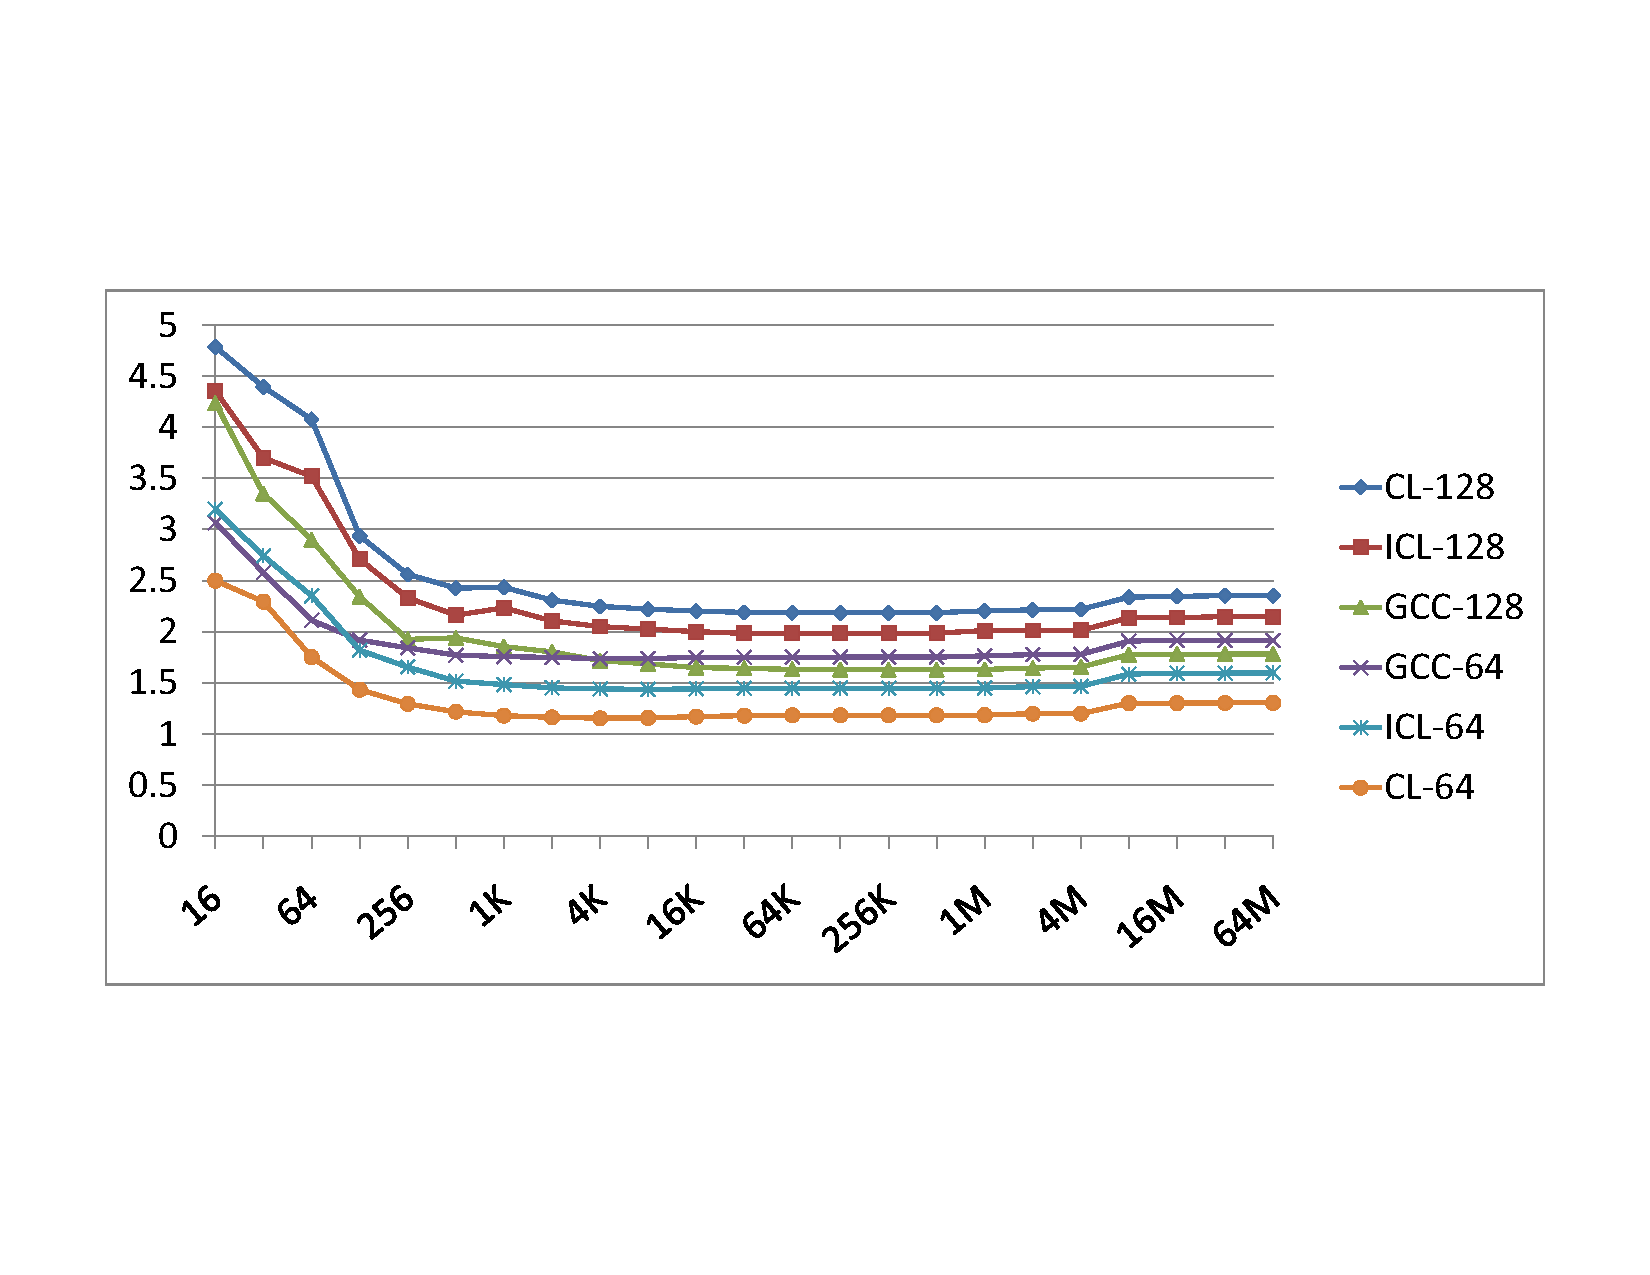
\includegraphics[trim=14.25mm 50mm 16.75mm 50mm, width=0.99\textwidth]{CompilerComparison.pdf} \label{f:CompilerComparison}
\end{center}

{\it``Multiword/$N$"} implements algorithm described in section
\ref{s:multiword} processing $N$ data streams in parallel in interleaved
manner.


\end{table}


% --------------------------------------
\begin{table}
\begin{center}

\caption{CRC-32 performance} \label{t:CRC32Perf}
\begin{tabular}{| l | c | c | c | c | c | c | c | c |}
  \hline
Input size           & 64    & 256   & 1K    & 4K    & 16K   & 64K   & 256K  & 1M       \\
  \hline
             Sarwate &  6.61 &  6.62 &  6.70 &  6.68 &  6.67 &  6.66 &  6.67 &  6.75    \\
               Black &  5.44 &  5.46 &  5.47 &  5.48 &  5.47 &  5.46 &  5.47 &  5.53    \\
             Slicing &  2.15 &  2.10 &  2.09 &  2.09 &  2.08 &  2.08 &  2.08 &  2.10    \\
         Blockword/3 &  2.27 &  2.14 &  2.15 &  2.13 &  2.13 &  1.55 &  1.39 &  1.31    \\
         Multiword/4 &  1.75 &  1.29 &  1.18 &  1.16 &  1.17 &  1.18 &  1.18 &  1.18    \\
  \hline
\end{tabular}
\end{center}

Number of CPU cycles per byte. 32-bit CRC (CRC-32C polynomial), 64-bit
platform, 64-bit tables, 64-bit reads (except Sarwate). Microsoft CL
15.00.30729 compiler. Warm data, warm tables.

\begin{center}
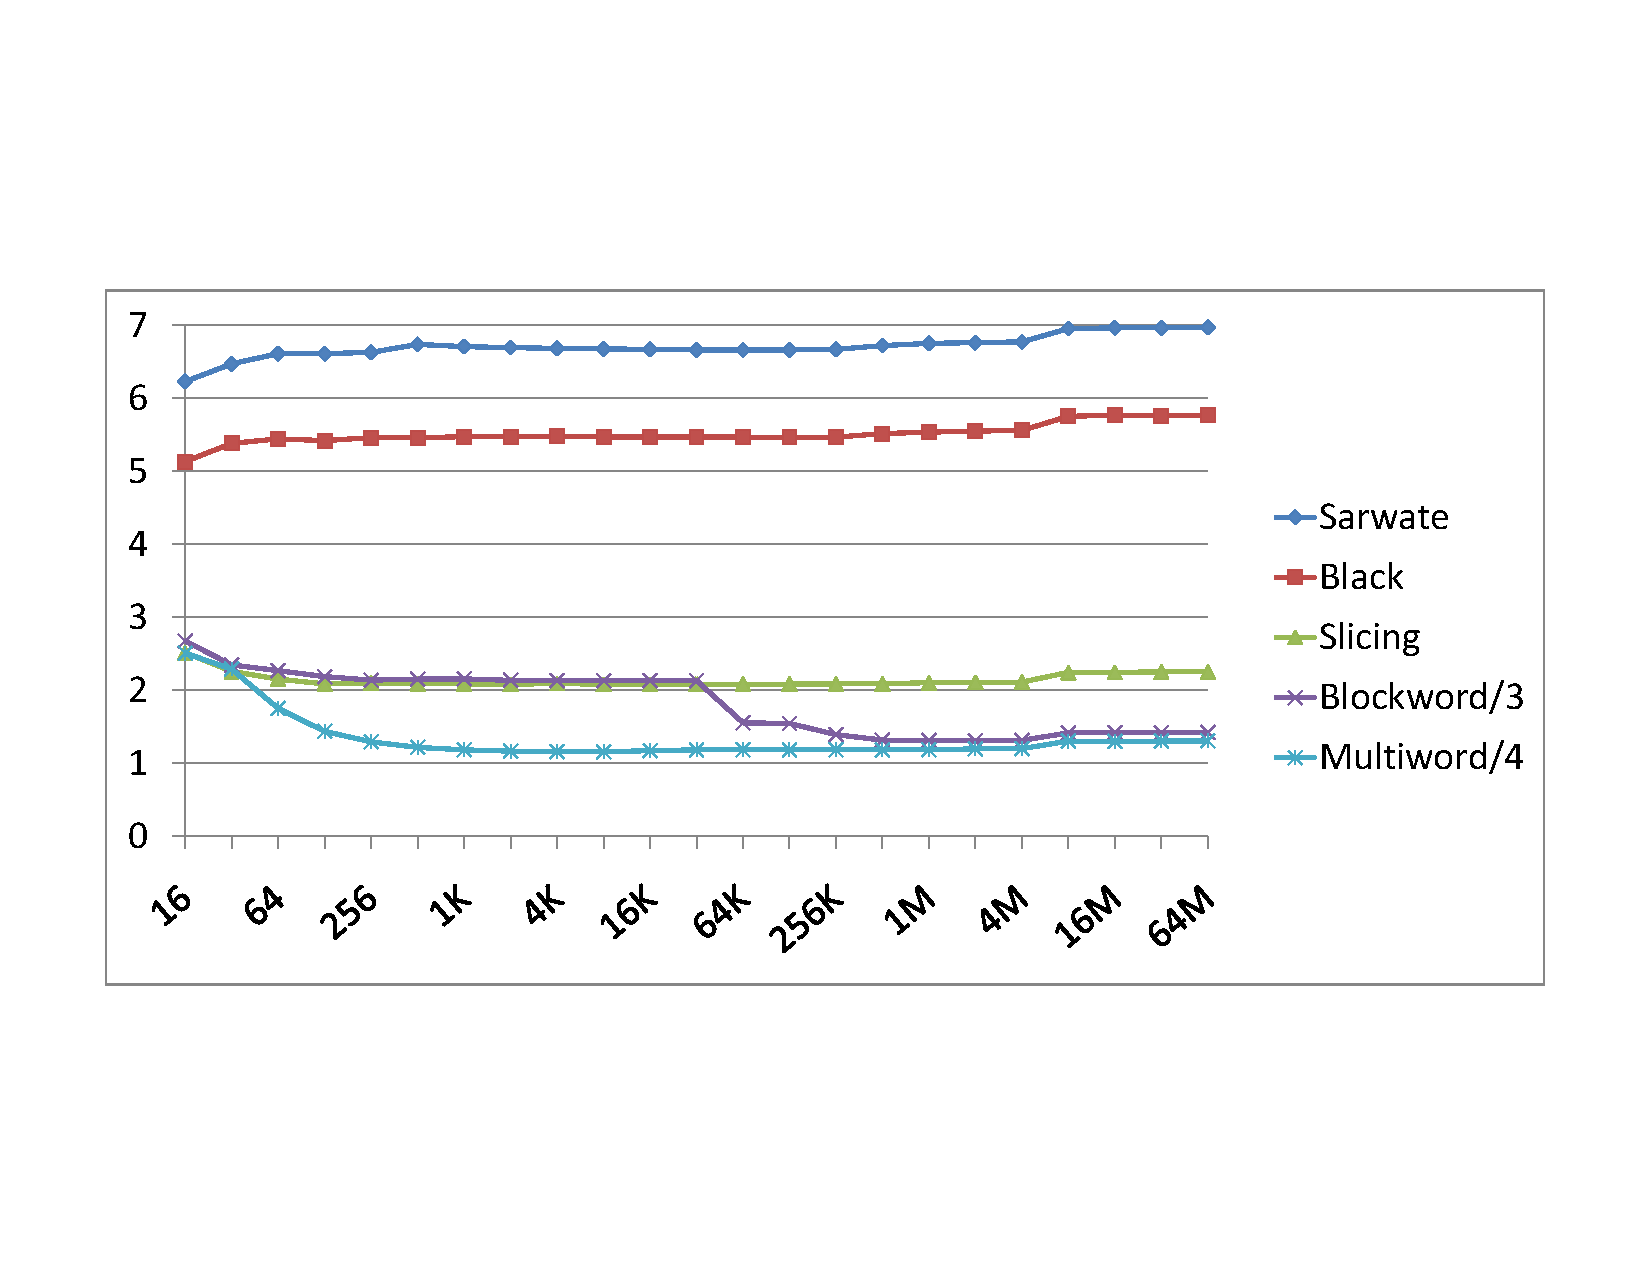
\includegraphics[trim=14.25mm 50mm 16.75mm 50mm, width=0.99\textwidth]{CRC32-full.pdf} \label{f:CRC32Perf}
\end{center}

{\it``Sarwate"} implements the algorithm described in section
\ref{s:crcbyte}.

{\it``Black"} implements the algorithm described in section
\ref{s:crcbyteword}.

{\it``Slicing"} implements the algorithm described in section
\ref{s:crcword}.

{\it``Blockword/3"} implements the algorithm described in section
\ref{s:blockword} with 3 stripes of 15,376 bytes each.

{\it``Multiword/4"} implements the algorithm described in section
\ref{s:multiword} processing 4 data streams in parallel in interleaved
manner.


\end{table}


% --------------------------------------
\begin{table}
\begin{center}

\caption{CRC-64 performance} \label{t:CRC64Perf}
\begin{tabular}{| l | c | c | c | c | c | c | c | c |}
  \hline
Input size           & 64    & 256   & 1K    & 4K    & 16K   & 64K   & 256K  & 1M       \\
  \hline
             Sarwate &  6.61 &  6.62 &  6.70 &  6.68 &  6.67 &  6.65 &  6.66 &  6.75    \\
               Black &  5.44 &  5.46 &  5.47 &  5.47 &  5.47 &  5.47 &  5.47 &  5.53    \\
             Slicing &  2.16 &  2.08 &  2.09 &  2.10 &  2.08 &  2.08 &  2.08 &  2.09    \\
         Blockword/3 &  2.27 &  2.14 &  2.15 &  2.13 &  2.13 &  1.59 &  1.41 &  1.33    \\
         Multiword/4 &  1.75 &  1.29 &  1.18 &  1.15 &  1.17 &  1.18 &  1.18 &  1.18    \\
  \hline
\end{tabular}
\end{center}

Number of CPU cycles per byte. 64-bit CRC (CRC-64-ECMA-182 polynomial),
64-bit platform, 64-bit tables, 64-bit reads (except Sarwate). Microsoft CL
15.00.30729 compiler. Warm data, warm tables.

\begin{center}
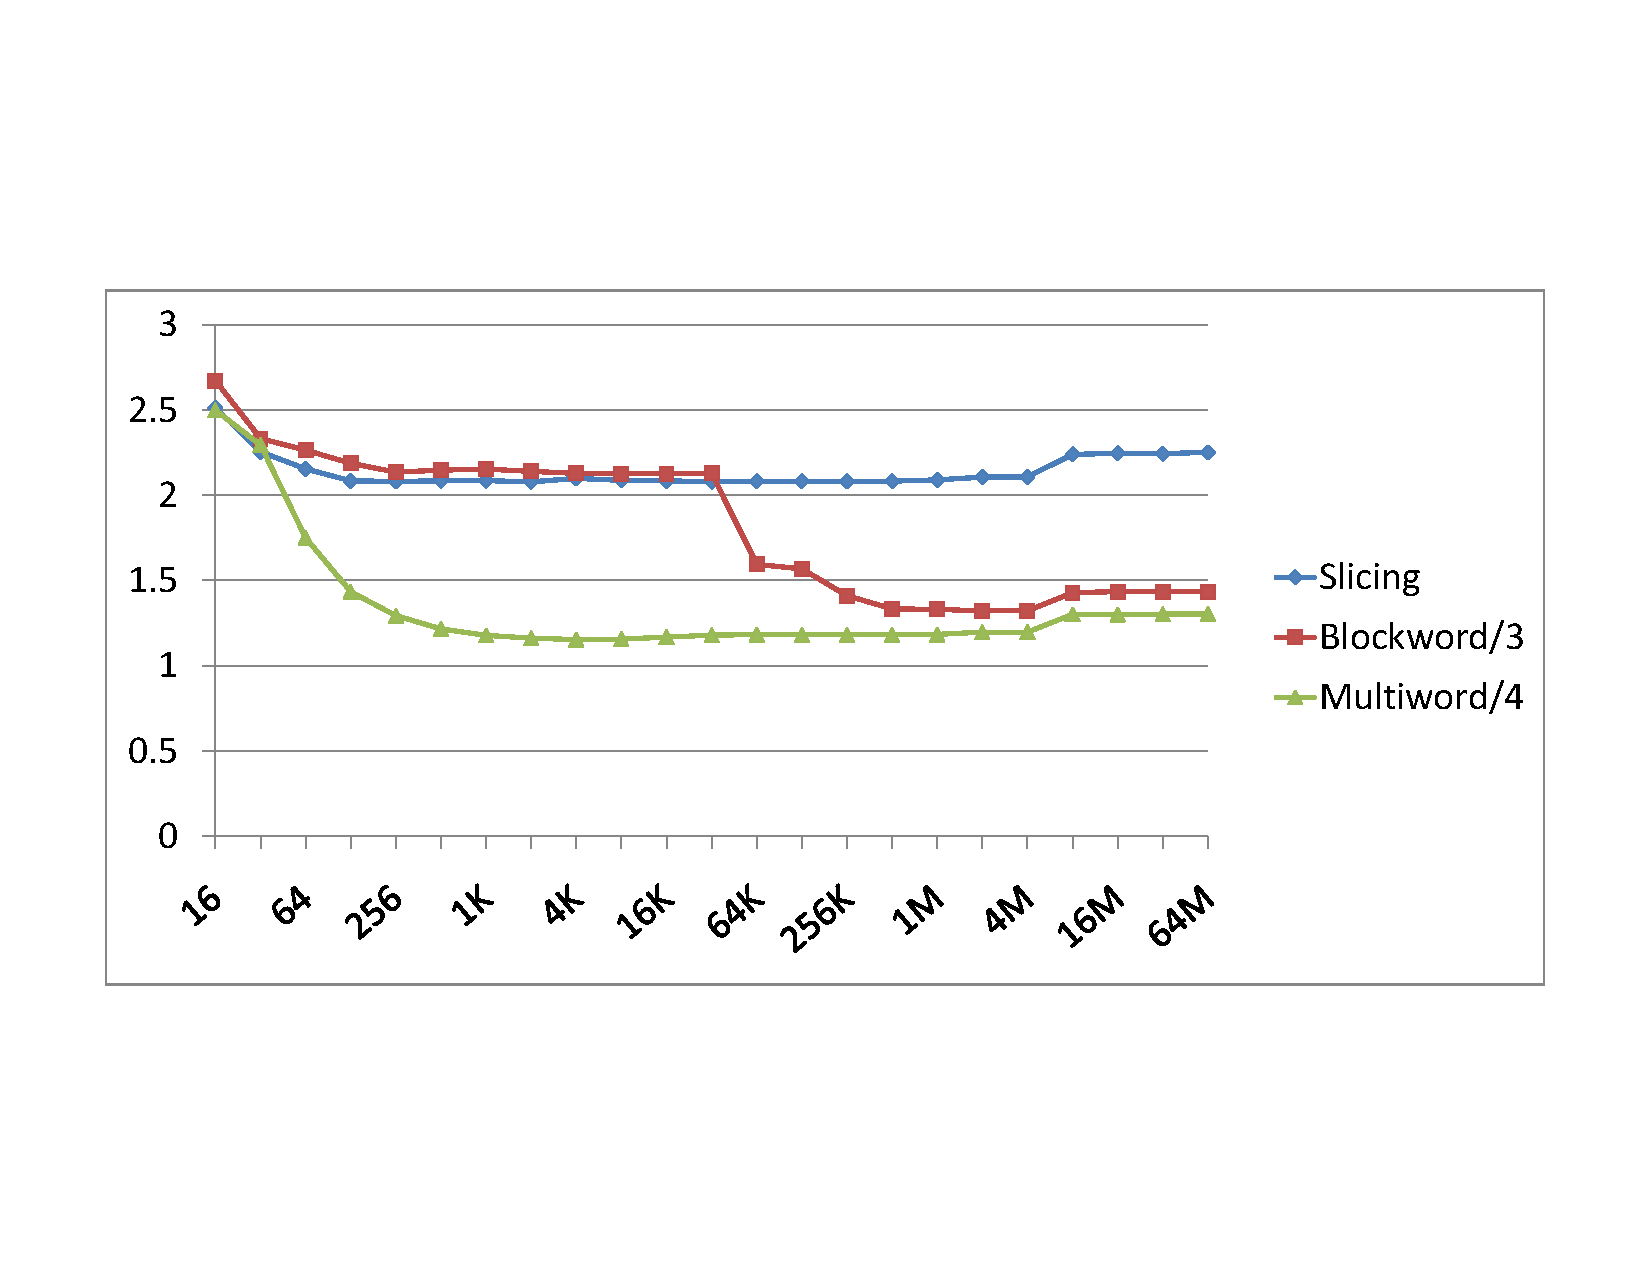
\includegraphics[trim=14.25mm 50mm 16.75mm 50mm, width=0.99\textwidth]{CRC64-small.pdf} \label{f:CRC64Perf}
\end{center}

{\it``Sarwate"} implements the algorithm described in section
\ref{s:crcbyte}.

{\it``Black"} implements the algorithm described in section
\ref{s:crcbyteword}.

{\it``Slicing"} implements the algorithm described in section
\ref{s:crcword}.

{\it``Blockword/3"} implements the algorithm described in section
\ref{s:blockword} with 3 stripes of 15,376 bytes each.

{\it``Multiword/4"} implements the algorithm described in section
\ref{s:multiword} processing 4 data streams in parallel in interleaved
manner.


\end{table}

% --------------------------------------
\begin{table}
\begin{center}


\caption{CRC-128 performance: Slicing CRC} \label{t:CRC128PerfSlicing}
\begin{tabular}{| l | c | c | c | c | c | c | c | c |}
  \hline
Input size   & 64    & 256   & 1K    & 4K    & 16K   & 64K   & 256K  & 1M       \\
  \hline
     CL/SSE2 &  4.02 &  3.81 &  4.01 &  4.05 &  4.13 &  4.18 &  4.20 &  4.24    \\
    ICL/SSE2 &  3.40 &  3.24 &  3.57 &  3.59 &  3.68 &  3.72 &  3.75 &  3.81    \\
    GCC/UINT &  3.45 &  3.24 &  3.36 &  3.48 &  3.61 &  3.64 &  3.67 &  3.72    \\
    GCC/SSE2 &  2.67 &  2.48 &  2.63 &  2.79 &  2.97 &  2.99 &  2.99 &  3.03    \\
  \hline
\end{tabular}


\caption{CRC-128 performance: Multiword CRC} \label{t:CRC128PerfMultiword}
\begin{tabular}{| l | c | c | c | c | c | c | c | c |}
  \hline
Input size & 64    & 256   & 1K    & 4K    & 16K   & 64K   & 256K  & 1M       \\
  \hline
GCC/UINT/3 &  3.83 &  3.02 &  3.04 &  3.01 &  3.00 &  2.98 &  2.98 &  3.00    \\
 CL/SSE2/5 &  4.08 &  2.56 &  2.43 &  2.25 &  2.20 &  2.19 &  2.18 &  2.20    \\
ICL/SSE2/5 &  3.52 &  2.33 &  2.23 &  2.05 &  2.00 &  1.99 &  1.99 &  2.01    \\
GCC/SSE2/6 &  2.90 &  1.93 &  1.85 &  1.72 &  1.65 &  1.63 &  1.63 &  1.63    \\
  \hline
\end{tabular}
\end{center}

Number of CPU cycles per byte. 128-bit CRC (CRC-128/IEEE polynomial),
64-bit platform, 128-bit tables, 64-bit reads. Warm data, warm tables.

All compilers were tested using SSE2 intrinsics (/SSE2 variants). GCC was
also tested using 128-bit integers provided by the compiler (GCC/UINT).

\begin{center}
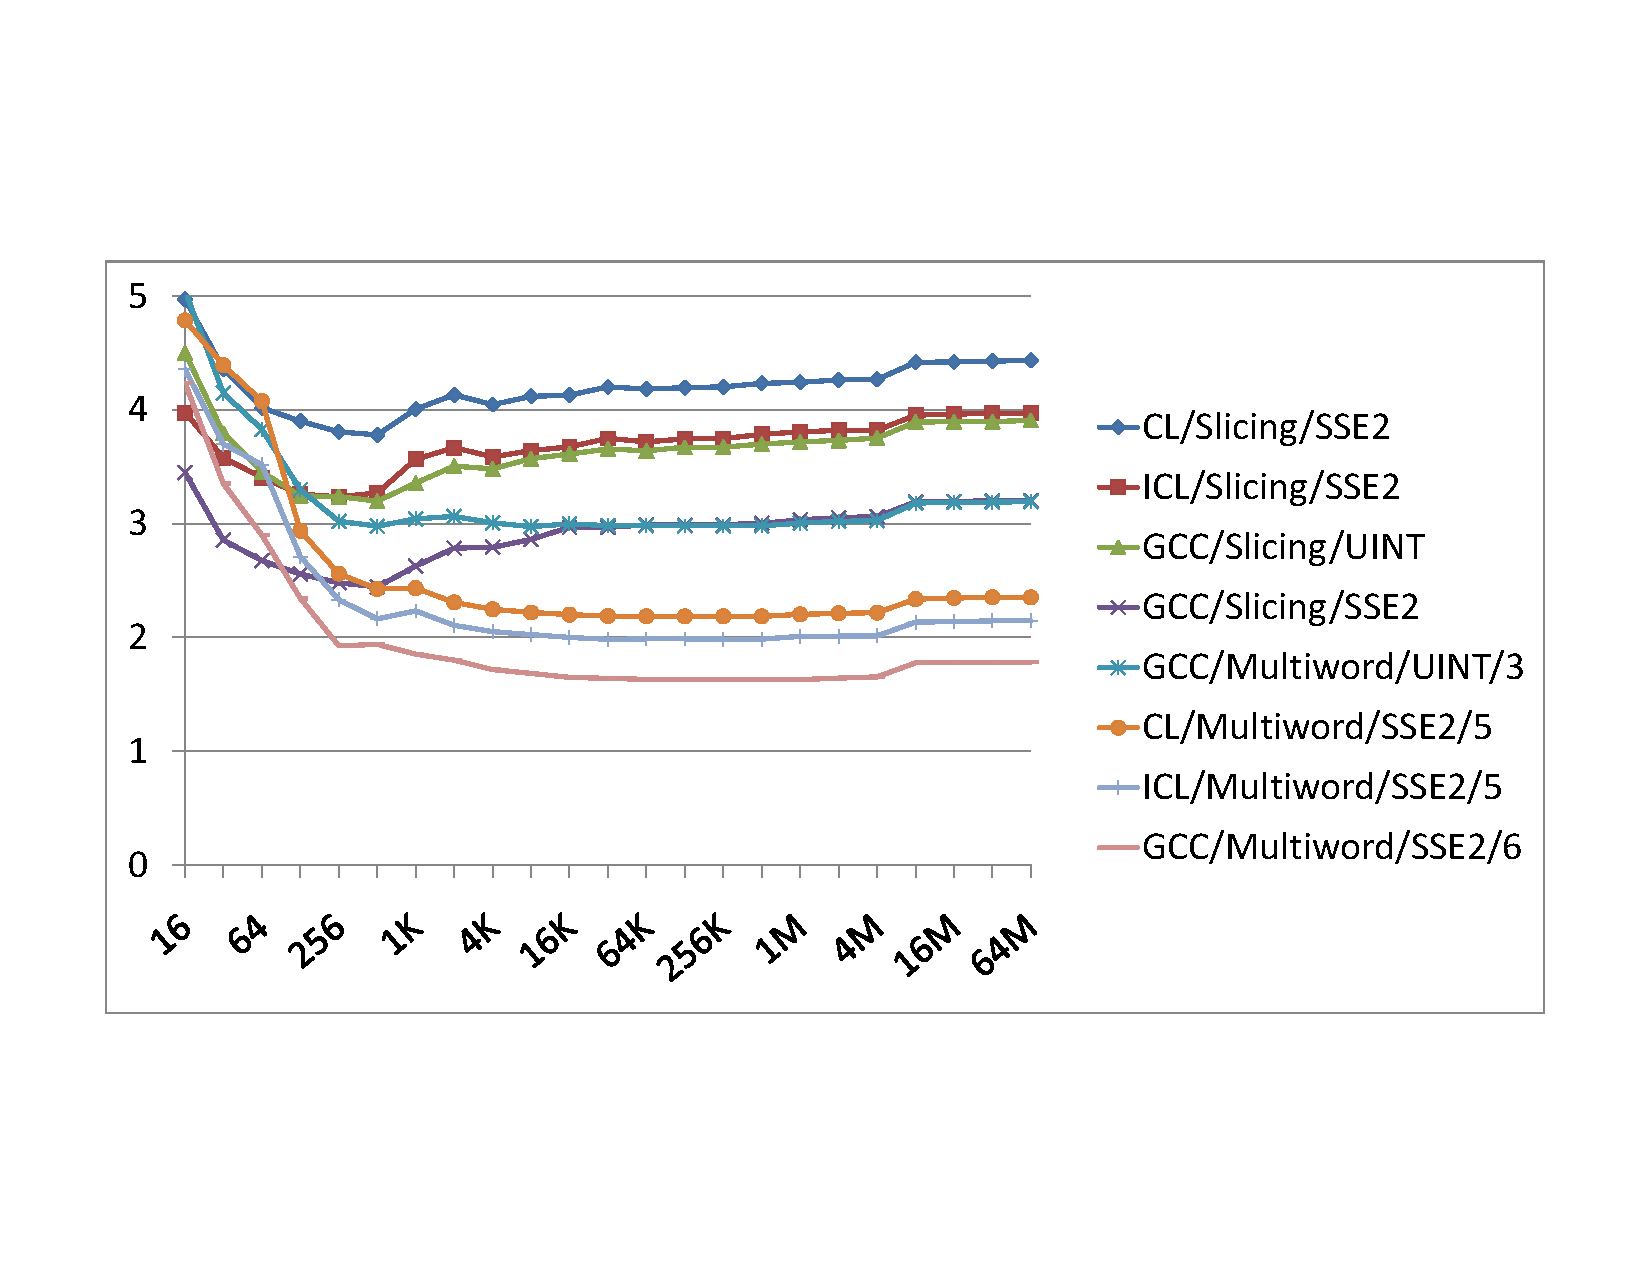
\includegraphics[trim=14.25mm 50mm 16.75mm 50mm, width=0.99\textwidth]{CRC128-full.pdf} \label{f:CRC128Perf}
\end{center}

{\it``Slicing"} implements algorithm described in section \ref{s:crcword}.

{\it``Multiword/$N$"} implements algorithm described in section
\ref{s:multiword} processing $N$ data streams in parallel in interleaved
manner. The optimal (for given compiler) value of $N$ was used.

\end{table}

\end{document}
